\RequirePackage{fix-cm}
\documentclass[smallextended]{svjour3}       % onecolumn (second format)
\smartqed  % flush right qed marks, e.g. at end of proof
\usepackage{graphicx,multicol,lipsum,caption,authblk}
\usepackage{amsmath,booktabs,verbatim,tikz}
\usepackage{geometry,pgf,pgfplots,}
\usepackage{mathptmx}
\usetikzlibrary{shapes.geometric, matrix,arrows,positioning,calc,intersections}
\begin{document}


\title{Stacking Sequence Optimization by an Improved Genetic Algorithm}
\titlerunning{Stacking Sequence Optimization}        % if too long for running head
\author{Zhang Huiyao$^1$  \and
	Atsushi Yokoyama $^{1,*}$
}
\authorrunning{Zhang Huiyao} % if too long for running head
\institute{Zhang Huiyao \at
              Room 203,Bulding 3,Kyoto Institue of Technology\\
			  Matsugasaki,Sakyo-ku,Kyoto,606-8585,JAPAN\\
              \email{zhanghy1012@gmail.com}           %  \\
           \and
           S. Author \at
              second address
}
\date{Received: date / Accepted: date}
\maketitle

\begin{abstract}
% 遗传算法
An improved genetic algorithm is used to obtain the stacking sequence of the laminate that reach the maximum strength
% BP神经网络


\keywords{Genetic Algorithm \and Laminates \and Stacking Sequence}
\end{abstract}

%\begin{multicols}{2}
%\begin{multicols}


\section{Introduction}
% 第一段
% 第一句话,FRP复合材料在众多领域都有着广泛的应用,因为它具有很高的强度比等性质.
Fiber-reinfored composites are widely used in automotive, aerospace, shipbuilding, and other branches of engineering because of their high specific strength and stiffness.
% 第二句话,复合材料层合板因为可以tailor,适合定制,所以它的优化策略就显得非常重要,fiber orientation, thickness and stacking sequence

% 第三句话,各种关于这种材料的优化都使用遗传算法

% 第二段
% 第一句介绍遗传算法
Genetic algorithms(GAs) simulate the process of natural evolutionary includes selection, crossover ,and mutation  according to Darwin's principal of "survival of the fittest".
% 第二句 列出最近几个遗传算法的应用

According to T Back \cite{back1994selective},the selection mechanism is one of the primary means of controlling the GA's convergence rate and its
likelihood of finding global optima.


Four evaluation criteria are used. 
The first is normalized cost per genetic search, $$C_{n}$$
cost is determinted by the following formula.

$$C_{n} = N_{g}P/R$$
where P is population size, R is Apparent reliability.




\section{Optimization formulation and solution}\label{sec:1}
Text with citations \cite{RefB} and \cite{RefJ}.
\subsection{Formulation}
For the orthotropic lamina, the strain-stress relation as:
\begin{equation}
    \begin{bmatrix}
        \sigma_1\\
        \sigma_2\\
        \tau_{12}
    \end{bmatrix}
    =
    \begin{bmatrix}
        Q_{11} & Q_{12} & 0\\
        Q_{12} & Q_{22} & 0\\
        0 & 0 & Q_{66}
    \end{bmatrix}
    \begin{bmatrix}
        \varepsilon_1\\
        \varepsilon_2\\
        \gamma
    \end{bmatrix}
\end{equation}
Where $Q_{ij}$ are the stiffnesses of the lamina that are related to the compliance matrix
compnents and elastic constants by
\begin{equation}
    \begin{split}
    &Q_{11}=\frac{E_1}{1-\mu_{12}\mu_{21}}\\
    &Q_{22}=\frac{E_2}{1-\mu_{12}\mu_{21}}\\
    &Q_{66}=G_{12}\\
    &Q_{12}=\frac{\mu_{21}E_2}{1-\mu_{12}\mu_{21}}\\
    \end{split}
\end{equation}
The transformation of the equation*sof the off-axis coordinates to the principal axis of the material stress tensor as
\begin{equation}
    [T]=
    \begin{bmatrix}
        \cos^2\theta & \sin^2\theta & 2\sin2\theta \\
        \sin^2\theta & \cos^2\theta & -2\sin2\theta \\
        -\frac{1}{2}\sin2\theta & \frac{1}{2}\sin2\theta & \cos2\theta
    \end{bmatrix}
\end{equation}

\begin{equation}
%	\begin{split}
	\begin{bmatrix}
		N_x \\
		N_y \\
		N_{xy}
	\end{bmatrix}
	=
	\begin{bmatrix}
		A_{11} & A_{12} & A_{16} \\
		A_{12} & A_{22} & A_{26} \\
		A_{16} & A_{26} & A_{66} 
	\end{bmatrix}
    \begin{bmatrix}
		\varepsilon_x^0 \\
        \varepsilon_y^0 \\
		\gamma_{xy}^0
    \end{bmatrix} \\
	+
	\begin{bmatrix}
		B_{11} & B_{12} & B_{16} \\
		B_{11} & B_{12} & B_{16} \\
		B_{16} & B_{26} & B_{66} 
	\end{bmatrix}
	\begin{bmatrix}
		k_x \\
		k_y \\
		k_{xy} 
	\end{bmatrix}
%	\end{split}
\end{equation}

\begin{equation*}
	%\begin{split}
	\begin{bmatrix}
		M_x \\
		M_y \\
		M_{xy}
	\end{bmatrix}
	=
	\begin{bmatrix}
		B_{11} & B_{12} & B_{16} \\
		B_{12} & B_{22} & B_{26} \\
		B_{16} & B_{26} & B_{66} 
	\end{bmatrix}
    \begin{bmatrix}
		\varepsilon_x^0 \\
        \varepsilon_y^0 \\
		\gamma_{xy}^0
    \end{bmatrix} \\
	+
	\begin{bmatrix}
		D_{11} & D_{12} & D_{16} \\
		D_{11} & D_{12} & D_{16} \\
		D_{16} & D_{26} & D_{66} 
	\end{bmatrix}
	\begin{bmatrix}
		k_x \\
		k_y \\
		k_{xy} 
	\end{bmatrix}
    %\end{split}
\end{equation*}

\begin{equation}
    \begin{split}
    &A_{ij}
	=
	\sum_{k=1}^n(\overline{Q_{ij}})_k(h_k-h_{k-1}) \\
    &B_{ij}
	=
	\frac{1}{2}\sum_{k=1}^n(\overline{Q_{ij}})_k(h_k-h_{k-1}) \\
    &D_{ij}
	=
	\frac{1}{3}\sum_{k=1}^n(\overline{Q_{ij}})_k(h_k-h_{k-1}) \\
    \end{split}
\end{equation}
\begin{equation}
    \begin{split}
    &F_{1}=\frac{1}{X_t}-\frac{1}{X_c},\quad  F_{11}=\frac{1}{X_tX_c} \\
    &F_{2}=\frac{1}{Y_t}-\frac{1}{Y_c},\quad  F_{22}=\frac{1}{Y_tY_c} \\
    &F_{66}=\frac{1}{S^2}
   \end{split}
\end{equation}

\begin{equation*}\label{strength-ratio}
    R=\frac{\sigma_{i(\alpha)}}{\sigma_i}
\end{equation*}
where $R$ is the strength ratio,$\sigma_{i{a}}$ is allowable stress,$\sigma_i$ is the stress under loading

substituting Eq.  \ref{strength-ratio} for $\sigma$ into Eq. \ref{Tsai-wu}, we obtain
\begin{equation*}
	\begin{split}
		F_1\sigma_{1(a)}&+F_2\sigma_{2(a)}+F_{11}\sigma_{1(a)}^2+F_{22}\sigma_{2(a)}^2 \\
						&+F_{66}\sigma_{6(a)}^2+2F_{12}\sigma_{1(a)}\sigma_{2(a)}=1
    \end{split}
\end{equation*}
For orthoropic materials with three planes of symmetry, 
\begin{equation*}\label{Tsai-wu}
	\begin{split}
		&(F_{11}\sigma_1^2+F_{22}\sigma_2^2+F_{66}\sigma_6^2+2F_{12}\sigma_1\sigma_2)R^2 \\
		&+(F_1\sigma_1+F_2\sigma_2)R-1=0 
    \end{split}
\end{equation*}
\subsection{fitness function}
The objective function to be maximized is the strenght of the laminate.
the ratio of the component of allowable stress and the stress component under stress.
\begin{equation*}\label{strength-ratio}
	F=max(\frac{1}{R(i)-1})
\end{equation*}
Substituting Eq. \ref{strength-ratio} for $R$ into Eq. \ref{Tsai-wu},we obtain
\begin{equation*}
	\begin{split}
		(F_{11}\sigma_1^2&+F_{22}\sigma_2^2+F_{66}\sigma_6^2+2F_{12}\sigma_1\sigma_2)R^2 \\
						 &+(F_1\sigma_1+F_2\sigma_2)R-1=0
	\end{split}
\end{equation*}



\subsection{Solution by a genetic algorithm}\label{sec:2}
as required. Don't forget to give each section
and subsection a unique label).




\section{Results and Discussion}

\captionof{table}{AS4C/PEEK Material Properties}
\begin{tabular}{ccc}
	\toprule
	Material& Parameter& Value\\
	\midrule
    1 & $E_x$/Gpa     & 141 \\
    2 & $E_y$/GPa     & 9.7 \\
    3 & $G_{xy}$/Gpa  & 5 \\
	4 & $X_t$/MPa     & 1732 \\
	5 & $X_c$/MPa     & 832 \\
	6 & $Y_t$/MPa     & 60 \\
	7 & $Y_c$/MPa     & 136 \\
	8 & S/MPa       & 113 \\
	\bottomrule
\end{tabular}



\captionof{table}{GA-parameters}
\begin{tabular}{cc}
	\toprule
	parameter & value \\
	\midrule
	population size      & 20               \\
    encoding method      & float encoding  \\
	selection strategy   & roulette wheel  \\
	crossover strategy   & one-point \\
	mutation strategy    & mass mutation   \\
	\bottomrule
\end{tabular}

\captionof{table}{Anneal Parameters}
\begin{tabular}{cc}
	\toprule
	parameter & value \\
	\midrule
    initial position & (10,10) \\
    initial temperature  &  25000 \\
	\bottomrule
\end{tabular}

\captionof{table}{Random Walk Algorithm}
\begin{tabular}{cc}
	\toprule
	parameter & value \\
	\midrule
    initial position & (10,10) \\
    initial step length &  0.5   \\
    number of random normalization vector & 1 \\
	\bottomrule
\end{tabular}



\captionof{table}{Improved Random Walk Algorithm}
\begin{tabular}{cc}
	\toprule
	parameter & value \\
	\midrule
    initial position & (10,10) \\
    initial step length &  10   \\
    number of random normalization vector & 10 \\
	\bottomrule
\end{tabular}





\section{Concluding Remarks}
\section{Acknowledgements}
This is work was supported by 
This is work was supported by 




\begin{center}
  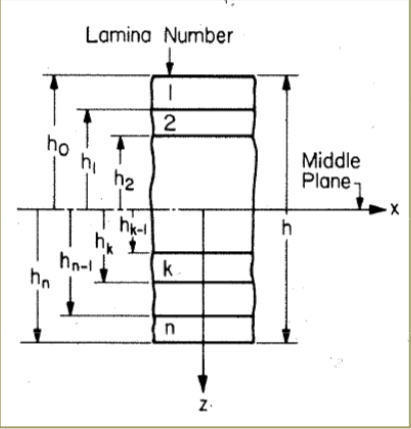
\includegraphics[width=\linewidth]{laminate.jpg}
  \captionof{figure}{Stacking Sequence Optimization }
\end{center}


%\end{multicols}
%\end{multicols}

The target function is 


\begin{equation}
p=\left\{
    \begin{array}{c}{1}  
        \text{      }   E\left(x_{n e w}\right)<E\left(x_{o l d}\right)
        \\ 
{\exp \left(-\frac{E\left(x_{new}\right)-E\left(x_{old}\right)}{T}\right)}
                        E\left(x_{n e w}\right)>E\left(x_{o l d}\right)
\end{array}\right.
\end{equation}


\begin{equation*}
    \begin{split}
        &f(r)=\sin(r)/r + 1  \\
             &\text{ where  } r=\sqrt{(x-50)^2+(y-50)^2}+2.71828
    \end{split}
\end{equation*}



For orthoropic materials with three planes of symmetry, 
\begin{equation}\label{Tsai-wu}
	\begin{split}
		F_1\sigma_1+F_2\sigma_2+F_{11}\sigma_1^2+F_{22}\sigma_2^2+F_{66}\sigma_6^2+2F_2F_2=1
    \end{split}
\end{equation}

we define $R$ is the strength ratio,
\begin{equation}\label{strength-ratio}
    R=\frac{\sigma_{i(\alpha)}}{\sigma_i}
\end{equation}
where $\sigma_{i{\sigma}}$ is allowable stress and $\sigma_i$ is the stress under loading,$R$ is
the ratio of the component of allowable stress and the stress component under stress.
substituting $\sigma_{i(\alpha)}$ for $\sigma_i$ into Eq. \ref{Tsai-wu}, we obtain
\begin{equation}
	\begin{split}
		F_1\sigma_{1(\alpha)}&+F_2\sigma_{2(\alpha)}+F_{11}\sigma_{1(\alpha)}^2+F_{22}\sigma_{2(\alpha)}^2 \\
						&+F_{66}\sigma_{6(\alpha)}^2+2F_{12}\sigma_{1(\alpha)}\sigma_{2(\alpha)}=1
    \end{split}
\end{equation}

Substituting $\sigma_{i(\sigma)}=R\sigma_i$  into Eq. \ref{Tsai-wu},we obtain
\begin{equation}
	\begin{split}
		(F_{11}\sigma_1^2&+F_{22}\sigma_2^2+F_{66}\sigma_6^2+2F_{12}\sigma_1\sigma_2)R^2 \\
						 &+(F_1\sigma_1+F_2\sigma_2)R-1=0
	\end{split}
\end{equation}
This is a quadric equation about $R$, the value of $(R-1)$ is the multiples that the stress can be increased              \\
The objective function to be maximized is the strenght of the laminate.
\begin{equation}
	F=max(\frac{1}{R(i)-1})
\end{equation}
where $i$ is the layer number


% 流程图
\tikzstyle{startstop} = [rectangle,rounded corners, minimum width=3cm,minimum height=1cm,text centered, draw=black,fill=white!30]
\tikzstyle{io} = [trapezium, trapezium left angle = 70,trapezium right angle=110,minimum width=3cm,minimum height=1cm,text centered,draw=black,fill=white!30]
\tikzstyle{process} = [rectangle,minimum width=6cm,minimum height=8mm,text centered,text width =6cm,draw=black,fill=white!30]
\tikzstyle{bp} = [rectangle,minimum width=6cm,minimum height=8mm,text centered,text width =4cm,draw=black,fill=white!30]
\tikzstyle{decision} = [diamond,minimum width=3cm,minimum height=1cm,text centered,draw=black,fill=white!30]
\tikzstyle{arrow} = [thick,->,>=stealth]

\begin{figure}
\centering
\begin{tikzpicture}[node distance=1.5cm]
\node (start) [startstop] {START};
\node (input1) [io,below of=start] {Create the initial population};
\node (process1) [process,below of=input1] {Evaluate the fitness of each individual};
% BP Neural Network
\node (bp) [bp,rotate=90, right of=process1, xshift=-6cm,yshift=-4cm] {Artificial Neural Network};
\node (process2) [process,below of=process1] {Select parents using roulette wheel};
\node (process3) [process,below of=process2] {Reproduce the children through crossover};
\node (process4) [process,below of=process3] {Check the children whether satisify requirement};
\node (process5) [process,below of=process4] {mutation};
\node (process6) [process,below of=process5] {Check the children whether satisify requirement};
\node (process7) [process,below of=process6] {Seek the individual of better fitness};
\node (process8) [process,below of=process7] {Produce new generation};
\node (process9) [process,below of=process8] {Check the number of generation};

%\node (decision1) [decision,below of=process1,yshift=-0.5cm] {Decession 1};
%\node (process2b) [process,right of =decision1,xshift=2cm] {Process 2b};
%\node (out1) [io,below of=process2a] {Output};
\node (stop) [startstop,below of=process9] {Stop};

%辅助框
%\draw[help lines,step=1cm,gray!20] (-5,-22) grid (5,5);

% 辅助点a
%\node (a) at (0,0) {a};
%\node (b) at (2,10) {b};
%\node (c) at (-2,3) {-b};
\draw [arrow] (start) -- (input1);
\draw [arrow] (input1) -- (process1);
\draw [arrow] (process1) -- (process2);
\draw [arrow] (process2) -- (process3);
\draw [arrow] (process3) -- (process4);
\draw [arrow] (process4) -- (process5);
\draw [arrow] (process5) -- (process6);
\draw [arrow] (process6) -- (process7);
\draw [arrow] (process7) -- (process8);
\draw [arrow] (process8) -- (process9);
%\draw [arrow] (process2decision1) -- node[anchor=east] {yes} (process2a);
%\draw [arrow] (decision1) -- node[anchor=south] {no} (process2b);
\draw [arrow] (process7) -| (bp);
\draw [arrow] (process1) -| (bp);
\draw [arrow] (process9) -- (stop);

% define a coordinate
\coordinate (below-start) at ($(input1.south)+(0,-0.25cm)$);
\draw [arrow] (process9.west) --  ++ (-1.0cm,0) |-  (below-start);

\end{tikzpicture}
\caption{the flowchart of Genetic Algorithm} \label{flowchart}
\end{figure}


% draw neural network



\bibliographystyle{plain}
\bibliography{citation-database}


\end{document}


